\section{The complex numbers}

\begin{outcome}
  \begin{enumerate}
  \item Understand the geometric significance of a complex number as a
    point in the plane.
  \item Prove algebraic properties of addition and multiplication of
    complex numbers, and apply these properties. Understand the action
    of taking the conjugate of a complex number.
  \item Understand the absolute value of a complex number and how to
    find it as well as its geometric significance.
  \end{enumerate}
\end{outcome}

\begin{definition}{The complex numbers}{complex-numbers}
  Let $i$ be an imaginary number such that $i\,^2=-1$. A \textbf{complex
    number}%
  \index{complex number} is a number of the form
  \begin{equation*}
    z = a + bi,
  \end{equation*}
  where $a$ and $b$ are real numbers. The set of all complex numbers
  is denoted $\C$.
\end{definition}

The form $z = a+bi$ is called the \textbf{standard form}%
\index{complex number!standard form}%
\index{standard form!of a complex number} or \textbf{Cartesian form}%
\index{complex number|Cartesian form}%
\index{Cartesian form!of a complex number} of the complex number $z$.
We refer to $a$ as the \textbf{real part}%
\index{complex number!real part}%
\index{real part!of a complex number} and to $b$ as the
\textbf{imaginary part}%
\index{complex number!imaginary part}%
\index{imaginary part!of a complex number} of $z$.

\textbf{Addition}%
\index{complex number!addition}%
\index{addition!of complex numbers}, \textbf{subtraction}%
\index{complex number!subtraction}%
\index{subtraction!of complex numbers}, and \textbf{multiplication}%
\index{complex number!multiplication}%
\index{multiplication!of complex numbers} of complex numbers are
defined in the obvious way, keeping in mind that $i\,^2=-1$. Namely, we
have
\begin{eqnarray*}
  (a+bi) + (c+di) &=& (a+c) + (b+d)i, \\
  (a+bi) - (c+di) &=& (a-c) + (b-d)i, \\
  (a+bi) (c+di)   &=& ac+adi+bci+bdi\,^2 ~=~ (ac-bd) + (ad + bc)i.
\end{eqnarray*}

\begin{example}{Addition, subtraction, and multiplication of complex numbers}{complex-add-subtract-multiply}
  \begin{itemize}
  \item $(3+5i) + (2-3i) = (3+2) + (5-3)i         = 5 + 2i$.
  \item $(3+5i) - (2-3i) = (3-2) + (5+3)i         = 1 + 8i$.
  \item $(3+5i) (2-3i)   = 6 - 9i + 10i - 15i\,^2 = 21 + i$.
  \end{itemize}
\end{example}

Division of complex numbers is more complicated. We first note that it
is easy to divide a complex number by a {\em real} number. Namely,
\begin{equation*}
  \frac{a+bi}{r} = \frac{a}{r} + \frac{b}{r}i.
\end{equation*}
But how can we divide by a complex number? We use the following
trick. Let $z=a+bi$ be a complex number, and consider the product
$(a+bi)(a-bi)$. It is equal to
\begin{equation*}
  (a+bi)(a-bi) = a^2 - b^2i\,^2 = a^2+b^2.
\end{equation*}
Therefore, $(a+bi)(a-bi)$ is always a {\em real} number, and therefore
easy to divide by. Therefore, we can compute the
\textbf{multiplicative inverse}%
\index{multipliciative inverse!of a complex number}%
\index{inverse!of a complex number}%
\index{complex number!inverse} of a complex number $z=a+bi$ as
follows:
\begin{equation*}
  z^{-1}
  = \frac{1}{z}
  = \frac{1}{a+bi}
  = \frac{1}{a+bi}\,\frac{a-bi}{a-bi}=\frac{a-bi}{a^{2}+b^{2}}.
\end{equation*}

\begin{example}{Inverse of a complex number}{complex-inverse}
  \begin{equation*}
    \frac{1}{2+5i}
    = \frac{2-5i}{2^2+5^2}
    = \frac{2}{29} - \frac{5}{29}i.
  \end{equation*}
\end{example}

\textbf{Division}\index{complex number!division}%
\index{division!of complex numbers} of complex numbers can then be
defined in terms of the multiplicative inverse, i.e.,
$\frac{z}{w} = zw^{-1}$.

\begin{example}{Division of complex numbers}{complex-division}
  \begin{equation*}
    \frac{5+7i}{3-4i}
    = \frac{(5+7i)(3+4i)}{(3-4i)(3+4i)}
    = \frac{-13+41i}{3^2+4^2}
    = -\frac{13}{25} + \frac{41}{25}i.
  \end{equation*}
\end{example}

As a special case of division, note that
\begin{equation*}
  i^{-1} = \frac{1}{i} = \frac{1(-i)}{i(-i)} = -i.
\end{equation*}

The complex numbers form a {\em field}, i.e., they satisfy the nine
field axioms. See Section~\ref{sec:fields} for the definition of a
field.

\begin{proposition}{The complex numbers form a field}{complex-field}
  The complex numbers, with the operations of addition, subtraction,
  multiplication, and division, form a {\em field}%
  \index{complex number!field axioms}%
  \index{field!of complex numbers}%
  \index{properties of addition!complex numbers}%
  \index{properties of multiplication!complex numbers}. Specifically,
  this means that they satisfy the following properties:
  \begin{itemize}
  \item[(A1)] {Commutative law of addition:} $z+w=w+z$;
  \item[(A2)] {Associative law of addition:} $(z+w)+u = z+(w+u)$;
  \item[(A3)] {Unit law of addition:} $0+z = z$;
  \item[(A4)] {Additive inverse:} $z+(-z)=0$;
  \item[(M1)] {Commutative law of multiplication:} $zw=wz$;
  \item[(M2)] {Associative law of multiplication:} $(zw)u=z(wu)$;
  \item[(M3)] {Unit law of multiplication:} $1z=z$;
  \item[(M4)] {Multiplicative inverse:} when $z$ is non-zero: $zz^{-1}=1$;
  \item[(D)] {Distributive law:} $z(w+u)=zw+zu$.
  \end{itemize}
\end{proposition}

Another useful operation on complex numbers is the complex
conjugate. Let $z = a+bi$ be a complex number. Then the
\textbf{conjugate}\index{complex number!conjugate}%
\index{conjugate!of a complex number}%
\index{complex conjugate} of $z$, written $\overline{z}$, is given by
\begin{equation*}
  \overline{z} = a-bi.
\end{equation*}
Note that if $z=a+bi$ is a complex number, then
$z\overline{z} = (a+bi)(a-bi) = a^2+b^2$. Therefore, $z\overline{z}$
is always a real number and $z\overline{z}\geq 0$. We define the
\textbf{magnitude}\index{complex number!magnitude}%
\index{magnitude!of a complex number} of $z$ to be
\begin{equation*}
  \abs{z} = \sqrt{z\overline{z}} = \sqrt{a^2+b^2}.
\end{equation*}
The magnitude is also sometimes called the \textbf{absolute
  value}\index{complex number!absolute value|see{magnitude}}%
\index{absolute value!of a complex number|see{magnitude}} or the
\textbf{modulus}\index{complex number!modulus|see{magnitude}}%
\index{modulus!of a complex number|see{magnitude}} of the complex
number.

\begin{example}{Conjugate and magnitude of a complex number}{complex-conjugate}
  \begin{itemize}
  \item $\overline{3+5i} = 3-5i$.
  \item $\overline{i} = -i$.
  \item $\overline{7} = 7$.
  \item $\abs{3+5i} = 3^2+5^2 = 34$.
  \item $\abs{i} = 1$.
  \item $\abs{-6} = 6$.
  \end{itemize}
\end{example}

Note that for a real number $a$, we have $\overline{a}=a$. Also, when
$a$ is real, the magnitude $|a| = \sqrt{a^2}$ is just the usual
absolute value of real numbers. The following two propositions
list some basic properties of the conjugate and of the magnitude.

\begin{proposition}{Properties of the conjugate}{properties-complex-conjugate}
  Let $z$ and $w$ be complex numbers. Then, the following properties
  of the conjugate hold.%
  \index{complex number!conjugate!properties}%
  \index{conjugate!of a complex number!properties}%
  \index{complex conjugate!properties}%
  \index{properties of complex conjugate}
  \begin{itemize}
  \item $\overline{z\pm w} = \overline{z} \pm \overline{w}$.
  \item $\overline{(zw)} = \overline{z}~ \overline{w}$.
  \item $\overline{z^{-1}} = \overline{z}^{-1}$.
  \item $\overline{z/w} = \overline{z} / \overline{w}$.
  \item $\overline{\overline{z}}=z$.
  \item $z$ is real if and only if $\overline{z}=z$.
  \end{itemize}
\end{proposition}

\begin{proposition}{Properties of the magnitude}{properties-complex-magnitude}
  Let $z,w$ be complex numbers.  The following properties hold.%
  \index{complex number!magnitude!properties}%
  \index{magnitude!of a complex number!properties}
  \begin{itemize}
  \item $\abs{z} \geq 0$, and $\abs{z}=0$ if and only if $z=0$.
  \item $\abs{zw} = \abs{z}\abs{w}$.
  \item $\abs{z+w} \leq \abs{z} +\abs{w}$.
  \end{itemize}
  The last of these properties is called the \textbf{triangle
    inequality}%
  \index{triangle inequality!of complex numbers}.
\end{proposition}

% ----------------------------------------------------------------------
\section{Geometric interpretation}

Just as a real number can be considered as a point on the line, a
complex number $z = a + bi$ can be considered as a point $(a,b)$ in
the plane whose $x$ coordinate is $a$ and whose $y$ coordinate is
$b$. For example, in the following picture, the complex number
$z = 3+2i$ can be represented as the point in the plane with
coordinates $(3,2)$.\index{complex number!geometric interpretation}

\begin{equation*}
  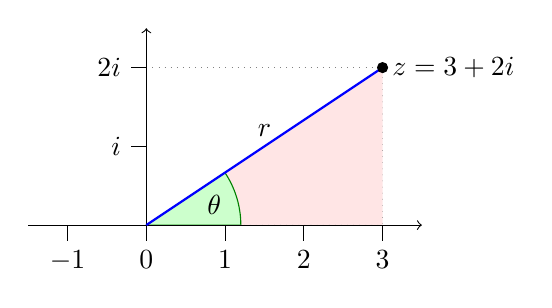
\begin{tikzpicture}
    \draw[help lines, dotted, fill=red!10] (0,0) -- (3,0) -- (3,2) -- cycle;
    \draw[help lines, dotted] (0,2) -- (3,2);
    \filldraw[fill=green!20,draw=green!50!black] (0,0) -- (1.2,0) arc (0:33.69:1.2) -- cycle;
    \node at (16.845:9mm){$\theta$};
    \draw[->](-1.5,0) -- (3.5,0);
    \draw[->](0,0) -- (0,2.5);
    \draw(0,1) -- +(-0.2,0) node[left] {$i$};
    \draw(0,2) -- +(-0.2,0) node[left] {$2i$};
    \draw(-1,0) -- +(0,-0.2) node[below] {$-1$};
    \draw(0,0) -- +(0,-0.2) node[below] {$0$};
    \draw(1,0) -- +(0,-0.2) node[below] {$1$};
    \draw(2,0) -- +(0,-0.2) node[below] {$2$};
    \draw(3,0) -- +(0,-0.2) node[below] {$3$};
    \draw[thick, blue] (0,0) -- node[above, black] {$r$} (3,2);
    \draw[fill, black] (3,2) circle [radius=1.8pt] node [right] {$z = 3+2i$};
  \end{tikzpicture}
\end{equation*}
The \textbf{magnitude}%
\index{complex number!magnitude}%
\index{magnitude!of a complex number} $r=\abs{z}$ of a complex number
is its distance from the origin. We also define the \textbf{argument}
of $z$ to be the angle $\theta$ between the $x$-axis and the line from
the origin to $z$, counted positively in the counterclockwise
direction. The magnitude $r$ and argument $\theta$ are shown in the
above picture.

Addition of complex numbers is like vector addition. The effect of
multiplying two complex numbers is to multiply their magnitudes and
add their arguments. For example, the following picture illustrates
the multiplication $(3+2i)(1+i)=1+5i$.
\begin{equation*}
  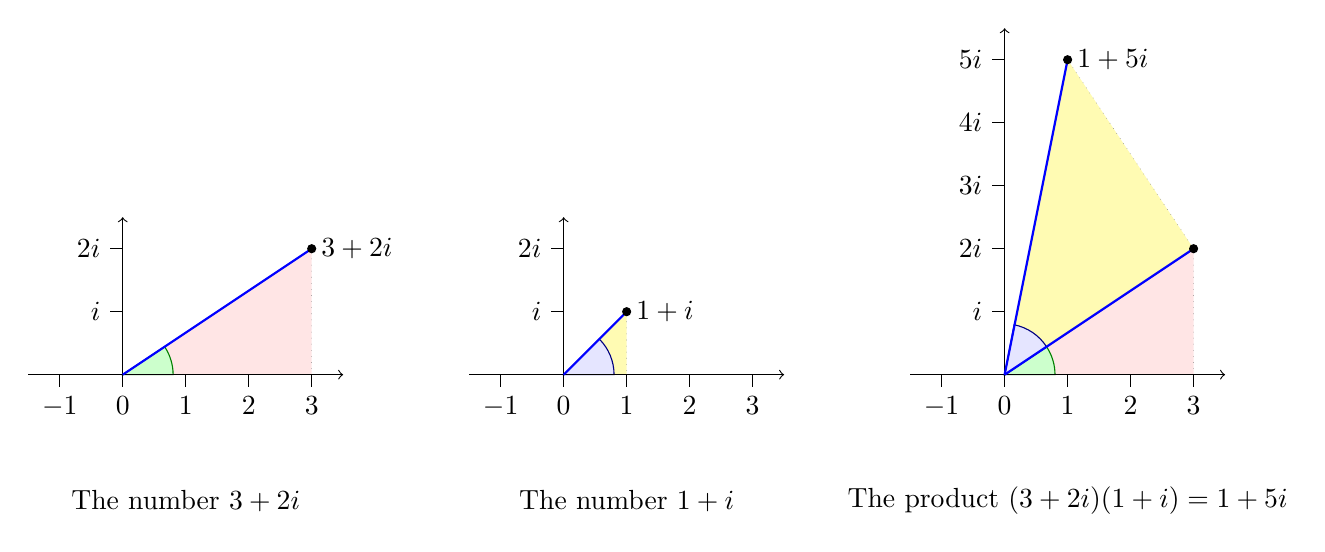
\begin{tikzpicture}[scale=0.8]
    \begin{scope}
      \draw[help lines, dotted, fill=red!10] (0,0) -- (3,0) -- (3,2) -- cycle;
      \filldraw[fill=green!20,draw=green!50!black] (0,0) -- (0.8,0) arc (0:33.69:0.8) -- cycle;
      \draw[->](-1.5,0) -- (3.5,0);
      \draw[->](0,0) -- (0,2.5);
      \draw(0,1) -- +(-0.2,0) node[left] {$i$};
      \draw(0,2) -- +(-0.2,0) node[left] {$2i$};
      \draw(-1,0) -- +(0,-0.2) node[below] {$-1$};
      \draw(0,0) -- +(0,-0.2) node[below] {$0$};
      \draw(1,0) -- +(0,-0.2) node[below] {$1$};
      \draw(2,0) -- +(0,-0.2) node[below] {$2$};
      \draw(3,0) -- +(0,-0.2) node[below] {$3$};
      \draw[thick, blue] (0,0) -- (3,2);
      \draw[fill, black] (3,2) circle [radius=1.8pt] node [right] {$3+2i$};
      \draw (1,-2) node {The number $3+2i$};
    \end{scope}
    \begin{scope}[xshift=7cm]
      \draw[help lines, dotted, fill=yellow!30] (0,0) -- (1,0) -- (1,1) -- cycle;
      \filldraw[fill=blue!10,draw=blue!50!black] (0,0) -- (0.8,0) arc (0:45:0.8) -- cycle;
      \draw[->](-1.5,0) -- (3.5,0);
      \draw[->](0,0) -- (0,2.5);
      \draw(0,1) -- +(-0.2,0) node[left] {$i$};
      \draw(0,2) -- +(-0.2,0) node[left] {$2i$};
      \draw(-1,0) -- +(0,-0.2) node[below] {$-1$};
      \draw(0,0) -- +(0,-0.2) node[below] {$0$};
      \draw(1,0) -- +(0,-0.2) node[below] {$1$};
      \draw(2,0) -- +(0,-0.2) node[below] {$2$};
      \draw(3,0) -- +(0,-0.2) node[below] {$3$};
      \draw[thick, blue] (0,0) -- (1,1);
      \draw[fill, black] (1,1) circle [radius=1.8pt] node [right] {$1+i$};
      \draw (1,-2) node {The number $1+i$};
    \end{scope}
    \begin{scope}[xshift=14cm]
      \draw[help lines, dotted, fill=red!10] (0,0) -- (3,0) -- (3,2) -- cycle;
      \draw[help lines, dotted, fill=yellow!30] (0,0) -- (3,2) -- (1,5) -- cycle;
      \filldraw[fill=green!20,draw=green!50!black] (0,0) -- (0.8,0) arc (0:33.69:0.8) -- cycle;
      \filldraw[fill=blue!10,draw=blue!50!black] (0,0) -- (33.69:0.8) arc (33:78.69:0.8) -- cycle;
      \draw[->](-1.5,0) -- (3.5,0);
      \draw[->](0,0) -- (0,5.5);
      \draw(0,1) -- +(-0.2,0) node[left] {$i$};
      \draw(0,2) -- +(-0.2,0) node[left] {$2i$};
      \draw(0,3) -- +(-0.2,0) node[left] {$3i$};
      \draw(0,4) -- +(-0.2,0) node[left] {$4i$};
      \draw(0,5) -- +(-0.2,0) node[left] {$5i$};
      \draw(-1,0) -- +(0,-0.2) node[below] {$-1$};
      \draw(0,0) -- +(0,-0.2) node[below] {$0$};
      \draw(1,0) -- +(0,-0.2) node[below] {$1$};
      \draw(2,0) -- +(0,-0.2) node[below] {$2$};
      \draw(3,0) -- +(0,-0.2) node[below] {$3$};
      \draw[thick, blue] (0,0) -- (3,2);
      \draw[fill, black] (3,2) circle [radius=1.8pt];
      \draw[thick, blue] (0,0) -- (1,5);
      \draw[fill, black] (1,5) circle [radius=1.8pt] node [right] {$1+5i$};
      \draw (1,-2) node {The product $(3+2i)(1+i)=1+5i$};
    \end{scope}
  \end{tikzpicture}
\end{equation*}
The effect of taking the complex conjugate is to reflect the given
complex number about the $x$ axis.

% ----------------------------------------------------------------------
\section{The fundamental theorem of algebra}

The complex numbers were invented so that equations such as $z^2+1=0$
would have solutions. In fact, this equation has two complex
solutions, namely $z=i$ and $z=-i$. However, something much more
general (and surprising) is true: {\em every} non-trivial polynomial
equation has a solution in the complex numbers. To understand this
statement, recall that a \textbf{polynomial}%
\index{polynomial} is an expression of the form
\begin{equation*}
  p(z) = a_nz^n + a_{n-1}z^{n-1} + \ldots + a_1z + a_0.
\end{equation*}
The constants $a_0,\ldots,a_n$ are called the \textbf{coefficients}%
\index{coefficient!of a polynomial}%
\index{polynomial!coefficient} of the polynomial. If $a_n$ is the
largest non-zero coefficient, we say that the polynomial has
\textbf{degree}%
\index{degree!of a polynomial}%
\index{polynomial!degree} $n$. A polynomial of degree $0$ is of the
form $p(z) = a_0$, and is also called a \textbf{constant polynomial}%
\index{polynomial!constant}%
\index{constant polynomial}. Recall that a \textbf{root}%
\index{root!of a polynomial}%
\index{polynomial!root} of a polynomial is a number $z$ such that
$p(z)=0$.  The fundamental theorem of algebra is the following:

\begin{theorem}{Fundamental theorem of algebra}{fundamental-algebra}
  Every non-constant polynomial $p(z)$ with real or complex
  coefficients has a complex root.
\end{theorem}

The proof of this theorem is beyond the scope of this book. Note that
the theorem does not say that the roots are always easy to find. To
find the roots of a polynomial of degree 2, we can use the quadratic
formula. However, if the degree is greater than 2, we may sometimes
have to use fancier methods, such as Newton's method from calculus, or
even a computer algebra system, to locate the roots. We give some
examples.

\begin{example}{Roots of a quadratic polynomial}{complex-root}
  Find the roots of the polynomial $p(z) = z^2 - 2z + 2$.
\end{example}

\begin{solution}
  The quadratic formula gives
  \begin{equation*}
    z = \frac{2 \pm \sqrt{-4}}{2}.
  \end{equation*}
  Of course, in the real numbers, the square root of $-4$ does not
  exist, so $p(z)$ has no roots in the real numbers. However, in the
  complex numbers, the square root of $-4$ exists and is equal to
  $\pm2i$. Thus, the roots of $p(z)$ are:
  \begin{equation*}
    z = \frac{2 \pm 2i}{2} = 1\pm i.
  \end{equation*}
  Indeed, we can double-check that $1+i$ and $1-i$ are in fact roots:
  \begin{equation*}
    \begin{array}{ll}
      p(1+i) = (1+i)^2 - 2(1+i) + 2 = (1 + 2i + (-1)) - 2 - 2i + 2 = 0, \\
      p(1-i) = (1-i)^2 - 2(1-i) + 2 = (1 - 2i + (-1)) - 2 + 2i + 2 = 0. \\
    \end{array}
  \end{equation*}
  \vspace{-2ex}
\end{solution}

\begin{example}{Roots of a cubic polynomial}{complex-root2}
  Find the roots of the polynomial $p(z) = z^3 - 4z^2 + 9z - 10$.
\end{example}

\begin{solution}
  By the intermediate value theorem of calculus, we know that a cubic
  polynomial with real coefficients always has at least one real
  root. This is because $p(z)$ goes to $-\infty$ when $z\to-\infty$
  and to $\infty$ when $z\to\infty$. By trial and error, we find that
  $z=2$ is a root of this polynomial. We can therefore factor out
  $(z-2)$ from this polynomial:
  \begin{equation*}
    p(z) = z^3 - 4z^2 + 9z - 10 = (z-2)(z^2 - 2z + 5).
  \end{equation*}
  Now we can use the quadratic formula to find the roots of $z^2 - 2z
  + 5$. We find
  \begin{equation*}
    z = \frac{2\pm\sqrt{-16}}{2} = \frac{2\pm 4i}{2} = 1\pm 2i.
  \end{equation*}
  Thus, the three complex roots of $p(z)$ are $z=2$, $z=1+2i$, and $z=1-2i$.
\end{solution}

The following proposition is an important and useful consequence of
the fundamental theorem of algebra:

\begin{proposition}{Factoring a polynomial}{complex-factoring}
  Let $p(z)$ be a polynomial of degree $n$ with real or complex
  coefficients. Then $p(z)$ can be factored into $n$ linear factors
  over the complex numbers, i.e., $p(z)$ can be written in the form
  \begin{equation*}
    p(z) = a(z-b_1)(z-b_2)\cdots(z-b_n),
  \end{equation*}
  where $b_1,\ldots,b_n$ are (not necessarily distinct) roots of
  $p(z)$.
\end{proposition}

\begin{proof}
  If $n=0$, then $p(z)=a$ and there is nothing to show. Otherwise, by
  the fundamental theorem of algebra, $p(z)$ has at least one complex
  root, say $b_1$. From calculus, we know that we can factor out
  $(z-b_1)$ from $p(z)$, i.e., we can find a polynomial $q(z)$ of
  degree $n-1$ such that 
  \begin{equation*}
    p(z) = (z-b_1) q(z),
  \end{equation*}
  We can repeatedly apply the same procedure to $q(z)$ until $p(z)$
  has been factored into linear factors.
\end{proof}

\begin{example}{Factoring a polynomial}
  Factor $p(z) = z^3 - 4z^2 + 9z - 10$ into linear factors.
\end{example}

\begin{solution}
  From Example~\ref{exa:complex-root2}, we know that $p(z)$ has three
  distinct roots $b_1=2$, $b_2=1+2i$, and $b_3=1-2i$. We can therefore
  write
  \begin{equation*}
    p(z) = a(z-b_1)(z-b_2)(z-b_3).
  \end{equation*}
  Since the leading term is $z^3$, we find that $a=1$. Therefore
  \begin{equation*}
    p(z) = (z-2)\,(z-1-2i)\,(z-1+2i).
  \end{equation*}
  \vspace{-2ex}
\end{solution}
